\documentclass{article}
\usepackage{amsmath}
\usepackage{amssymb}
\usepackage{graphicx}
\usepackage{hyperref}
\usepackage[version=4]{mhchem}


\begin{document}
(AMC) In circle \(O\) chord \(A B\) is produced so that \(B C\) equals a radius of the circle. \(C O\) is drawn and extended to \(D . A O\) is drawn. Which of the following expresses the relationship between angles \(x\) and \(y\) ?\\
(A) \(x=3 y\)\\
(B) \(x=2 y\)\\
(C) \(x=60^{\circ}\)\\
(D) there is no special relationship between \(x\) and \(y\) or \(x=3 y\), depending upon the length of \(A B\).\\
(E) \(x=2 y\)\\
\centering
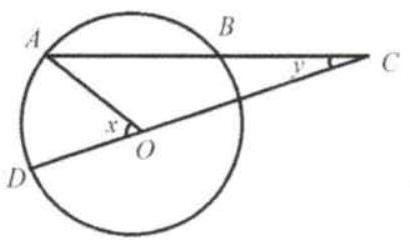
\includegraphics[width=\textwidth]{images/150(2).jpg}

Solution: (A).


Connect \(O B\).\\
Since \(O B=B C, \angle B O C=\angle B C O=y\).\\
Since \(\angle O B A\) is the exterior angle of \(\triangle O B C, \angle O B A=2 y\).\\
Since \(O B=O A, \angle O A B=\angle O B A=2 y\).\\
\centering
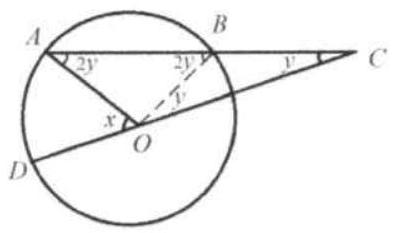
\includegraphics[width=\textwidth]{images/151(2).jpg}\\
since \(\angle A O D\) is the exterior angle of \(\triangle A O C, \angle A O D=2 y\) \(+y=3 y\).


\end{document}
